%%% Local Variables:
%%% mode: latex
%%% TeX-master: "../cheat-sheet"
%%% End:

\subsubsection*{Memory}

\begin{itemize}
\item How is the memory in a computer typically organized?
  \begin{enumerate}
    \item How is it addressed?
    \item How does it look like to the processor?
    \item What memory areas do a program use?
    \item How are they laid out? In what order? Where in memory?
    \item Single threaded

  \end{enumerate}
\end{itemize}

\paragraph{Answer}
\begin{enumerate}
  \item By a pointer of the given type.
  \item Like a one dimensional list of integers.
  \item Heap and stack.
  \item In address-space see voluntary, in memory use shot gun.
\end{enumerate}


\subsubsection*{Memory I}

Where do
\begin{enumerate}
\item Global variables go?
\item How is it addressed?
\item How does it look like to the processor?
\end{enumerate}

\paragraph{Answer}
\begin{enumerate}
  \item Global variables are stored on the heap
  \item See figure~\ref{fig:stack-heap} for organization
\end{enumerate}

\begin{figure}[H]
  \centering
  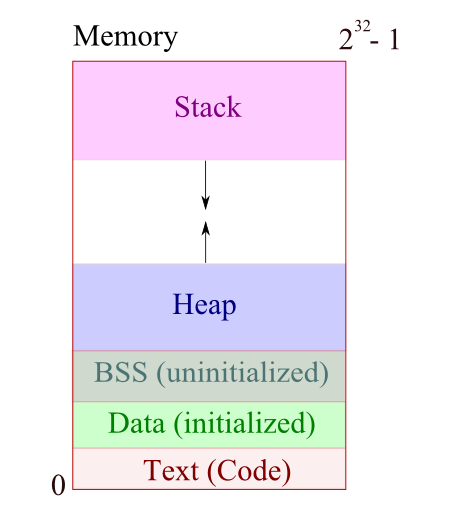
\includegraphics[scale=0.6]{images/memory_diagram}
  \caption{Memory diagram}
\label{fig:stack-heap}
\end{figure}

\subsubsection*{Pointers}

\begin{itemize}
\item Fundamentally, what is a pointer?
\item How is it represented?
\item How many bits are used?
\item Is type associated with pointers?
\item How do you do type casting?
\end{itemize}

\paragraph{Answer}

\begin{itemize}
\item  Fundamentally, pointers are represented as the smallest integer which can hold an address
– Describes an address and how to interpretate it
\item Represented using the (*) symbol. E.g. {\tt char *string; }
\item Size of pointer equals usually (Windownz) system's \texttt{word} size
\item Like this: {\tt ppi = (double *) pn; /* pn originally of type (int *) */ }
\end{itemize}
